\section{Odd One Out Learning}

Odd-one-out uses temporal ordering for representation learning in self supervised way.
This network is a new way to learn visual features for videos without using category level annotations. This method is applied to self supervised video representation learning where they sample sub sequences from videos and ask the network to learn to predict the odd video sequence. Here the odd video sub sequence is sampled such that it has wrong temporal order of frames while the even ones have the correct temporal order. 
They transfer weights to action recognition and fine tune on supervised set and show improvement over fully supervised learning.

Given $(N+1)$ number of sub sequenced videos from one single video, $N$ are in correct chronological order of frames which is the even set. The odd set consist of frame sampled from invalid sub sequenced video. One out of $(N+1)$ elements is odd object.

Furthermore the position of the odd element is randomized by shuffling sequence permutation.
Thus the odd one out prediction task reduces to an $(N+1)$ way classification problem, which can be solved by maximum likelihood estimation. 

The Model :  MultiBranch Convolutional neural Network consist of $(N+1)$ input branches. 
Each contain 5 Convolutional layers. 
The fusion layer -- merges the information from $(N+1)$ branches after the first fully connected layer. And helps to find regularities and pick the element with irregularities. The two approaches are used are Concatenation Model and Sum of difference. Which is shown in figure fusionmodel.

Video Frame Encoding: Each sub video is encoded to extract temporal information before presentation to the network. As we want the network to learn video representation by exploiting the structure of sequences. 

A single RGB image wont have the information about the previous and next frames. For encoding the motion, they are using sum of difference, stack of difference and dynamic images.

Sum of Difference : In this method they are taking the difference of frames and then summing the difference to obtain a single image. Here the single image captures the structure of the sequences. 
It is similar to weighted average of frames.

Dynamic Images: In this method they are pre processing the images before doing the sum of difference approach and obtain a smoothed sequence.
It can be computed fast as a weighted linear combination of original frames.

Stack of Difference: To capture the motion and dynamics of short video clips stack of difference of frames is taken. 


\begin{figure*}
\centering
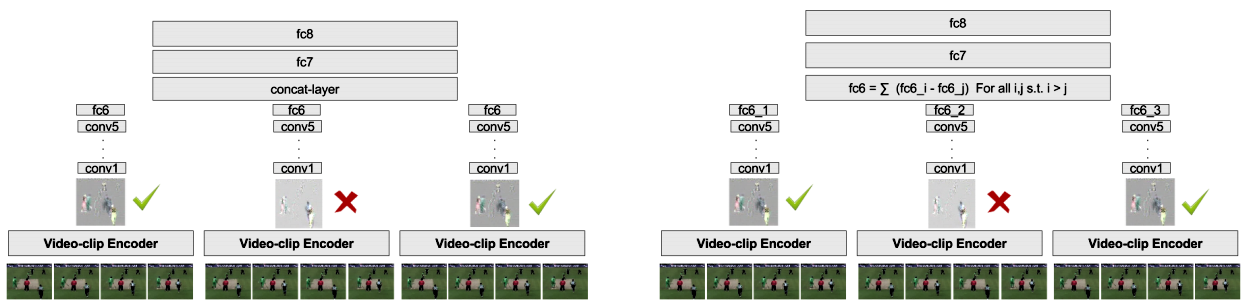
\includegraphics[width=\textwidth]{images/o3n1.png}
\caption{Concatenation Model and Sum of Difference Model}
\label{fig:fusionmodel}
\end{figure*}
